%% fig_f3primereach.tex   (generated by make_round19.py; do not edit by hand)
%% Where (F3') and the Hodge conjecture are known by arguments on zero-cycles and rationally connected fibrations.
\documentclass[tikz,border=8pt]{standalone}
\usepackage{amsmath,amssymb}
\usetikzlibrary{arrows.meta,calc,decorations.pathreplacing}
%% palette.tex -- shared colour definitions for the figures
\definecolor{PInk}{RGB}{26,32,44}
\definecolor{PBlue}{RGB}{37,82,139}
\definecolor{PTeal}{RGB}{23,127,125}
\definecolor{POchre}{RGB}{193,138,44}
\definecolor{PClay}{RGB}{178,74,58}
\definecolor{PSlate}{RGB}{108,122,137}
\definecolor{PViolet}{RGB}{110,86,150}
\definecolor{WBlue}{RGB}{223,234,246}
\definecolor{WTeal}{RGB}{220,238,236}
\definecolor{WOchre}{RGB}{250,240,218}
\definecolor{WClay}{RGB}{247,229,224}
\definecolor{WSlate}{RGB}{238,241,244}
\definecolor{PMag}{RGB}{158,58,110}
\definecolor{PGrass}{RGB}{62,124,66}
\definecolor{PAmber}{RGB}{214,112,38}
\definecolor{PIndigo}{RGB}{58,64,140}
\definecolor{PRule}{RGB}{176,186,197}

%% shared macros so the standalone figures match the paper
\providecommand{\QQ}{\mathbb{Q}}
\providecommand{\ZZ}{\mathbb{Z}}
\providecommand{\RR}{\mathbb{R}}
\providecommand{\CC}{\mathbb{C}}
\providecommand{\PP}{\mathbb{P}}
\providecommand{\Kx}{K^{\times}}
\providecommand{\HW}{W}
\providecommand{\Nm}{\mathrm{N}}
\providecommand{\Hdg}{\mathrm{Hdg}}
\providecommand{\NS}{\mathrm{NS}}
\providecommand{\cA}{\mathcal{A}}
\providecommand{\cD}{\mathcal{D}}
\providecommand{\cF}{\mathcal{F}}
\providecommand{\cP}{\mathcal{P}}
\providecommand{\cO}{\mathcal{O}}
\providecommand{\cQ}{\mathcal{Q}}
\providecommand{\bbar}[1]{\overline{#1}}
\providecommand{\ch}{\operatorname{ch}}
\providecommand{\End}{\mathrm{End}}
\providecommand{\Ext}{\operatorname{Ext}}
\providecommand{\Supp}{\operatorname{Supp}}

\begin{document}
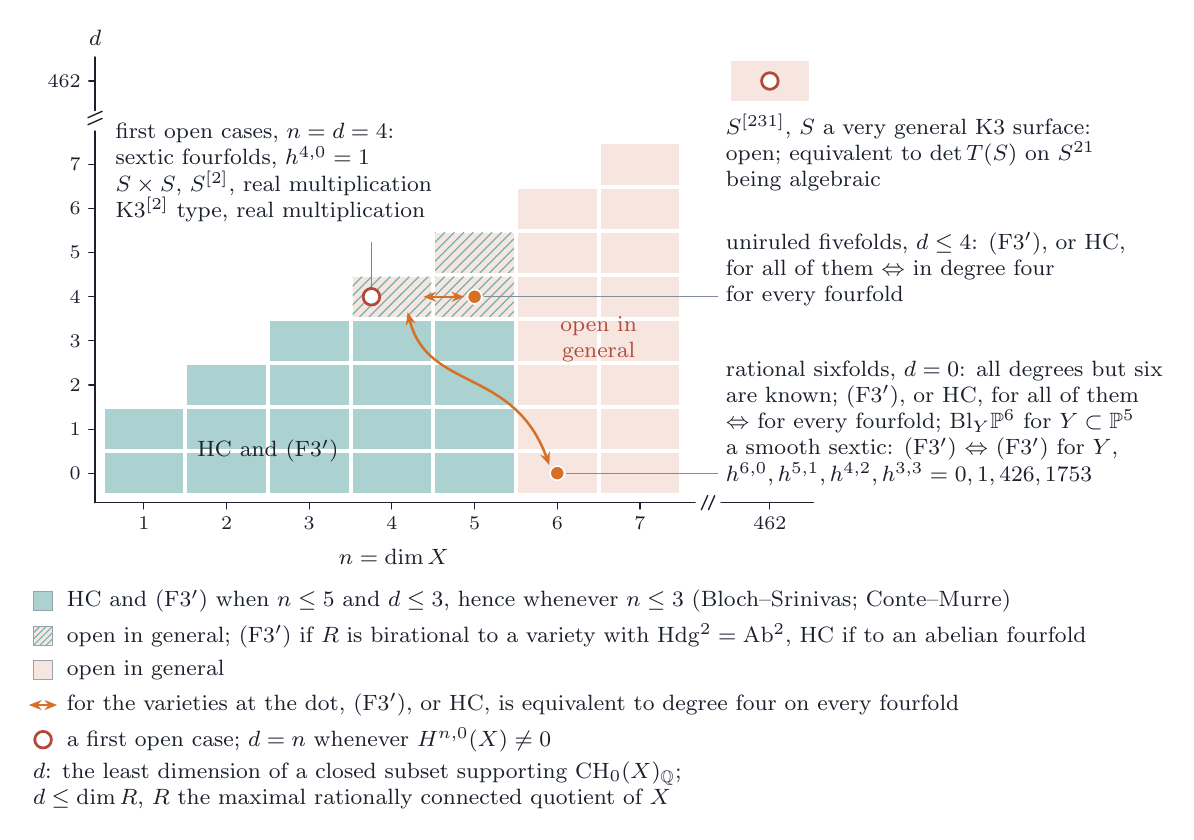
\begin{tikzpicture}[x=1cm,y=1cm,line join=round,line cap=round,
  font=\small,text=PInk,lbl/.style={inner sep=1pt}]
  \path[fill=PTeal!36!white,draw=none] (0.0000,0.0000) rectangle (1.0000,0.5100);
  \path[fill=PTeal!36!white,draw=none] (0.0000,0.5600) rectangle (1.0000,1.0700);
  \path[fill=PTeal!36!white,draw=none] (1.0500,0.0000) rectangle (2.0500,0.5100);
  \path[fill=PTeal!36!white,draw=none] (1.0500,0.5600) rectangle (2.0500,1.0700);
  \path[fill=PTeal!36!white,draw=none] (1.0500,1.1200) rectangle (2.0500,1.6300);
  \path[fill=PTeal!36!white,draw=none] (2.1000,0.0000) rectangle (3.1000,0.5100);
  \path[fill=PTeal!36!white,draw=none] (2.1000,0.5600) rectangle (3.1000,1.0700);
  \path[fill=PTeal!36!white,draw=none] (2.1000,1.1200) rectangle (3.1000,1.6300);
  \path[fill=PTeal!36!white,draw=none] (2.1000,1.6800) rectangle (3.1000,2.1900);
  \path[fill=PTeal!36!white,draw=none] (3.1500,0.0000) rectangle (4.1500,0.5100);
  \path[fill=PTeal!36!white,draw=none] (3.1500,0.5600) rectangle (4.1500,1.0700);
  \path[fill=PTeal!36!white,draw=none] (3.1500,1.1200) rectangle (4.1500,1.6300);
  \path[fill=PTeal!36!white,draw=none] (3.1500,1.6800) rectangle (4.1500,2.1900);
  \path[fill=WClay,draw=none] (3.1500,2.2400) rectangle (4.1500,2.7500);
  \begin{scope}\clip (3.1500,2.2400) rectangle (4.1500,2.7500);\draw[PTeal!60,line width=0.45pt] (2.6400,2.2400) -- (3.1500,2.7500) (2.7600,2.2400) -- (3.2700,2.7500) (2.8800,2.2400) -- (3.3900,2.7500) (3.0000,2.2400) -- (3.5100,2.7500) (3.1200,2.2400) -- (3.6300,2.7500) (3.2400,2.2400) -- (3.7500,2.7500) (3.3600,2.2400) -- (3.8700,2.7500) (3.4800,2.2400) -- (3.9900,2.7500) (3.6000,2.2400) -- (4.1100,2.7500) (3.7200,2.2400) -- (4.2300,2.7500) (3.8400,2.2400) -- (4.3500,2.7500) (3.9600,2.2400) -- (4.4700,2.7500) (4.0800,2.2400) -- (4.5900,2.7500);\end{scope}
  \path[fill=PTeal!36!white,draw=none] (4.2000,0.0000) rectangle (5.2000,0.5100);
  \path[fill=PTeal!36!white,draw=none] (4.2000,0.5600) rectangle (5.2000,1.0700);
  \path[fill=PTeal!36!white,draw=none] (4.2000,1.1200) rectangle (5.2000,1.6300);
  \path[fill=PTeal!36!white,draw=none] (4.2000,1.6800) rectangle (5.2000,2.1900);
  \path[fill=WClay,draw=none] (4.2000,2.2400) rectangle (5.2000,2.7500);
  \begin{scope}\clip (4.2000,2.2400) rectangle (5.2000,2.7500);\draw[PTeal!60,line width=0.45pt] (3.6900,2.2400) -- (4.2000,2.7500) (3.8100,2.2400) -- (4.3200,2.7500) (3.9300,2.2400) -- (4.4400,2.7500) (4.0500,2.2400) -- (4.5600,2.7500) (4.1700,2.2400) -- (4.6800,2.7500) (4.2900,2.2400) -- (4.8000,2.7500) (4.4100,2.2400) -- (4.9200,2.7500) (4.5300,2.2400) -- (5.0400,2.7500) (4.6500,2.2400) -- (5.1600,2.7500) (4.7700,2.2400) -- (5.2800,2.7500) (4.8900,2.2400) -- (5.4000,2.7500) (5.0100,2.2400) -- (5.5200,2.7500) (5.1300,2.2400) -- (5.6400,2.7500);\end{scope}
  \path[fill=WClay,draw=none] (4.2000,2.8000) rectangle (5.2000,3.3100);
  \begin{scope}\clip (4.2000,2.8000) rectangle (5.2000,3.3100);\draw[PTeal!60,line width=0.45pt] (3.6900,2.8000) -- (4.2000,3.3100) (3.8100,2.8000) -- (4.3200,3.3100) (3.9300,2.8000) -- (4.4400,3.3100) (4.0500,2.8000) -- (4.5600,3.3100) (4.1700,2.8000) -- (4.6800,3.3100) (4.2900,2.8000) -- (4.8000,3.3100) (4.4100,2.8000) -- (4.9200,3.3100) (4.5300,2.8000) -- (5.0400,3.3100) (4.6500,2.8000) -- (5.1600,3.3100) (4.7700,2.8000) -- (5.2800,3.3100) (4.8900,2.8000) -- (5.4000,3.3100) (5.0100,2.8000) -- (5.5200,3.3100) (5.1300,2.8000) -- (5.6400,3.3100);\end{scope}
  \path[fill=WClay,draw=none] (5.2500,0.0000) rectangle (6.2500,0.5100);
  \path[fill=WClay,draw=none] (5.2500,0.5600) rectangle (6.2500,1.0700);
  \path[fill=WClay,draw=none] (5.2500,1.1200) rectangle (6.2500,1.6300);
  \path[fill=WClay,draw=none] (5.2500,1.6800) rectangle (6.2500,2.1900);
  \path[fill=WClay,draw=none] (5.2500,2.2400) rectangle (6.2500,2.7500);
  \path[fill=WClay,draw=none] (5.2500,2.8000) rectangle (6.2500,3.3100);
  \path[fill=WClay,draw=none] (5.2500,3.3600) rectangle (6.2500,3.8700);
  \path[fill=WClay,draw=none] (6.3000,0.0000) rectangle (7.3000,0.5100);
  \path[fill=WClay,draw=none] (6.3000,0.5600) rectangle (7.3000,1.0700);
  \path[fill=WClay,draw=none] (6.3000,1.1200) rectangle (7.3000,1.6300);
  \path[fill=WClay,draw=none] (6.3000,1.6800) rectangle (7.3000,2.1900);
  \path[fill=WClay,draw=none] (6.3000,2.2400) rectangle (7.3000,2.7500);
  \path[fill=WClay,draw=none] (6.3000,2.8000) rectangle (7.3000,3.3100);
  \path[fill=WClay,draw=none] (6.3000,3.3600) rectangle (7.3000,3.8700);
  \path[fill=WClay,draw=none] (6.3000,3.9200) rectangle (7.3000,4.4300);
  \path[fill=WClay,draw=none] (7.9500,4.9800) rectangle (8.9500,5.4900);
  \draw[PInk,line width=0.5pt] (-0.1200,-0.1200) -- (7.5000,-0.1200);
  \draw[PInk,line width=0.5pt] (7.8300,-0.1200) -- (9.0000,-0.1200);
  \draw[PInk,line width=0.5pt] (-0.1200,-0.1200) -- (-0.1200,4.6000);
  \draw[PInk,line width=0.5pt] (-0.1200,4.8600) -- (-0.1200,5.5400);
  \draw[PInk,line width=0.5pt] (7.5800,-0.2100) -- (7.6600,-0.0300);
  \draw[PInk,line width=0.5pt] (7.6700,-0.2100) -- (7.7500,-0.0300);
  \draw[PInk,line width=0.5pt] (-0.2100,4.6800) -- (-0.0300,4.7600);
  \draw[PInk,line width=0.5pt] (-0.2100,4.7700) -- (-0.0300,4.8500);
  \draw[PInk,line width=0.4pt] (0.5000,-0.1200) -- (0.5000,-0.2000);
  \draw[PInk,line width=0.4pt] (1.5500,-0.1200) -- (1.5500,-0.2000);
  \draw[PInk,line width=0.4pt] (2.6000,-0.1200) -- (2.6000,-0.2000);
  \draw[PInk,line width=0.4pt] (3.6500,-0.1200) -- (3.6500,-0.2000);
  \draw[PInk,line width=0.4pt] (4.7000,-0.1200) -- (4.7000,-0.2000);
  \draw[PInk,line width=0.4pt] (5.7500,-0.1200) -- (5.7500,-0.2000);
  \draw[PInk,line width=0.4pt] (6.8000,-0.1200) -- (6.8000,-0.2000);
  \draw[PInk,line width=0.4pt] (8.4500,-0.1200) -- (8.4500,-0.2000);
  \draw[PInk,line width=0.4pt] (-0.1200,0.2550) -- (-0.2000,0.2550);
  \draw[PInk,line width=0.4pt] (-0.1200,0.8150) -- (-0.2000,0.8150);
  \draw[PInk,line width=0.4pt] (-0.1200,1.3750) -- (-0.2000,1.3750);
  \draw[PInk,line width=0.4pt] (-0.1200,1.9350) -- (-0.2000,1.9350);
  \draw[PInk,line width=0.4pt] (-0.1200,2.4950) -- (-0.2000,2.4950);
  \draw[PInk,line width=0.4pt] (-0.1200,3.0550) -- (-0.2000,3.0550);
  \draw[PInk,line width=0.4pt] (-0.1200,3.6150) -- (-0.2000,3.6150);
  \draw[PInk,line width=0.4pt] (-0.1200,4.1750) -- (-0.2000,4.1750);
  \draw[PInk,line width=0.4pt] (-0.1200,5.2350) -- (-0.2000,5.2350);
  \draw[PAmber,line width=0.9pt,{Stealth[length=4.6pt,width=3.6pt]}-{Stealth[length=4.6pt,width=3.6pt]}] (4.5700,2.4950) -- (4.0500,2.4950);
  \draw[PAmber,line width=0.9pt,{Stealth[length=4.6pt,width=3.6pt]}-{Stealth[length=4.6pt,width=3.6pt]}] (5.6500,0.3550) .. controls (5.2000,1.6050) and (4.1000,1.2900) .. (3.8500,2.3000);
  \path[fill=PAmber,draw=white,line width=0.60pt] (4.7000,2.4950) circle (2.60pt);
  \path[fill=PAmber,draw=white,line width=0.60pt] (5.7500,0.2550) circle (2.60pt);
  \path[fill=white,draw=PClay,line width=1.00pt] (3.3900,2.4950) circle (3.00pt);
  \path[fill=white,draw=PClay,line width=1.00pt] (8.4500,5.2350) circle (3.00pt);
  \path[fill=PTeal!36!white,draw=PSlate!70,line width=0.35pt] (-0.9000,-1.4900) rectangle (-0.6600,-1.2500);
  \path[fill=WClay,draw=PSlate!70,line width=0.35pt] (-0.9000,-1.9300) rectangle (-0.6600,-1.6900);
  \begin{scope}\clip (-0.9000,-1.9300) rectangle (-0.6600,-1.6900);\draw[PTeal!60,line width=0.40pt] (-1.1400,-1.9300) -- (-0.9000,-1.6900) (-1.0600,-1.9300) -- (-0.8200,-1.6900) (-0.9800,-1.9300) -- (-0.7400,-1.6900) (-0.9000,-1.9300) -- (-0.6600,-1.6900) (-0.8200,-1.9300) -- (-0.5800,-1.6900) (-0.7400,-1.9300) -- (-0.5000,-1.6900) (-0.6600,-1.9300) -- (-0.4200,-1.6900);\end{scope}
  \path[fill=WClay,draw=PSlate!70,line width=0.35pt] (-0.9000,-2.3700) rectangle (-0.6600,-2.1300);
  \draw[PAmber,line width=0.9pt,{Stealth[length=4.6pt,width=3.6pt]}-{Stealth[length=4.6pt,width=3.6pt]}] (-0.9600,-2.6900) -- (-0.6000,-2.6900);
  \path[fill=white,draw=PClay,line width=1.00pt] (-0.7800,-3.1300) circle (3.00pt);
  \draw[PClay!80,line width=0.45pt] (3.3900,3.1850) -- (3.3900,2.6250);
  \draw[PSlate!85,line width=0.35pt] (7.7900,2.4950) -- (4.8200,2.4950);
  \draw[PSlate!85,line width=0.35pt] (7.7900,0.2550) -- (5.8700,0.2550);
  \node[lbl,text=PInk,font=\footnotesize] at (2.0750,0.5350) {$\mathrm{HC}$ and (F3$'$)};
  \node[lbl,text=PClay,font=\footnotesize,align=center] at (6.2750,1.9600) {open in\\general};
  \node[lbl,anchor=north,text=PInk,font=\scriptsize] at (0.5000,-0.2600) {$1$};
  \node[lbl,anchor=north,text=PInk,font=\scriptsize] at (1.5500,-0.2600) {$2$};
  \node[lbl,anchor=north,text=PInk,font=\scriptsize] at (2.6000,-0.2600) {$3$};
  \node[lbl,anchor=north,text=PInk,font=\scriptsize] at (3.6500,-0.2600) {$4$};
  \node[lbl,anchor=north,text=PInk,font=\scriptsize] at (4.7000,-0.2600) {$5$};
  \node[lbl,anchor=north,text=PInk,font=\scriptsize] at (5.7500,-0.2600) {$6$};
  \node[lbl,anchor=north,text=PInk,font=\scriptsize] at (6.8000,-0.2600) {$7$};
  \node[lbl,anchor=north,text=PInk,font=\scriptsize] at (8.4500,-0.2600) {$462$};
  \node[lbl,anchor=east,text=PInk,font=\scriptsize] at (-0.2600,0.2550) {$0$};
  \node[lbl,anchor=east,text=PInk,font=\scriptsize] at (-0.2600,0.8150) {$1$};
  \node[lbl,anchor=east,text=PInk,font=\scriptsize] at (-0.2600,1.3750) {$2$};
  \node[lbl,anchor=east,text=PInk,font=\scriptsize] at (-0.2600,1.9350) {$3$};
  \node[lbl,anchor=east,text=PInk,font=\scriptsize] at (-0.2600,2.4950) {$4$};
  \node[lbl,anchor=east,text=PInk,font=\scriptsize] at (-0.2600,3.0550) {$5$};
  \node[lbl,anchor=east,text=PInk,font=\scriptsize] at (-0.2600,3.6150) {$6$};
  \node[lbl,anchor=east,text=PInk,font=\scriptsize] at (-0.2600,4.1750) {$7$};
  \node[lbl,anchor=east,text=PInk,font=\scriptsize] at (-0.2600,5.2350) {$462$};
  \node[lbl,anchor=north,text=PInk,font=\footnotesize] at (3.6750,-0.6700) {$n=\dim X$};
  \node[lbl,anchor=south,text=PInk,font=\footnotesize] at (-0.1200,5.6400) {$d$};
  \node[lbl,anchor=west,text=PInk,font=\footnotesize,align=left] at (0.1000,4.0720) {first open cases, $n=d=4$:\\sextic fourfolds, $h^{4,0}=1$\\$S\times S$, $S^{[2]}$, real multiplication\\K3$^{[2]}$ type, real multiplication};
  \node[lbl,anchor=west,text=PInk,font=\footnotesize,align=left] at (7.8500,4.3279) {$S^{[231]}$, $S$ a very general K3 surface:\\open; equivalent to $\det T(S)$ on $S^{21}$\\being algebraic};
  \node[lbl,anchor=west,text=PInk,font=\footnotesize,align=left] at (7.8500,2.8466) {uniruled fivefolds, $d\le4$: (F3$'$), or $\mathrm{HC}$,\\for all of them $\Leftrightarrow$ in degree four\\for every fourfold};
  \node[lbl,anchor=west,text=PInk,font=\footnotesize,align=left] at (7.8500,0.8899) {rational sixfolds, $d=0$: all degrees but six\\are known; (F3$'$), or $\mathrm{HC}$, for all of them\\$\Leftrightarrow$ for every fourfold; $\mathrm{Bl}_{Y}\PP^{6}$ for $Y\subset\PP^{5}$\\a smooth sextic: (F3$'$) $\Leftrightarrow$ (F3$'$) for $Y$,\\$h^{6,0},h^{5,1},h^{4,2},h^{3,3}=0,1,426,1753$};
  \node[lbl,anchor=west,text=PInk,font=\footnotesize] at (-0.5200,-1.3700) {$\mathrm{HC}$ and (F3$'$) when $n\le5$ and $d\le3$, hence whenever $n\le3$ (Bloch--Srinivas; Conte--Murre)};
  \node[lbl,anchor=west,text=PInk,font=\footnotesize] at (-0.5200,-1.8100) {open in general; (F3$'$) if $R$ is birational to a variety with $\Hdg^{2}=\mathrm{Ab}^{2}$, $\mathrm{HC}$ if to an abelian fourfold};
  \node[lbl,anchor=west,text=PInk,font=\footnotesize] at (-0.5200,-2.2500) {open in general};
  \node[lbl,anchor=west,text=PInk,font=\footnotesize] at (-0.5200,-2.6900) {for the varieties at the dot, (F3$'$), or $\mathrm{HC}$, is equivalent to degree four on every fourfold};
  \node[lbl,anchor=west,text=PInk,font=\footnotesize] at (-0.5200,-3.1300) {a first open case; $d=n$ whenever $H^{n,0}(X)\neq0$};
  \node[lbl,anchor=west,text=PInk,font=\footnotesize,align=left] at (-0.9500,-3.7119) {$d$: the least dimension of a closed subset supporting $\mathrm{CH}_{0}(X)_{\QQ}$;\\$d\le\dim R$, $R$ the maximal rationally connected quotient of $X$};
\end{tikzpicture}
\end{document}
